%& /home/adi/.config/emacs/.local/cache/org/persist/2e/543a70-8c42-4823-a991-bb8bb3325e32-6794375529a5c50db9caf3bdeb15d0a4
% Created 2025-02-19 Wed 11:21
% Intended LaTeX compiler: pdflatex
\documentclass[a4paper,11pt,twoside]{article}
\usepackage[utf8]{inputenc}
\usepackage[T1]{fontenc}
\usepackage{amsmath}
\usepackage{amssymb}
\usepackage{capt-of}
\usepackage{hyperref}
\usepackage{booktabs}
\usepackage{xcolor}
\usepackage{colortbl}
\usepackage{siunitx}
\usepackage{tabu}
\usepackage{etoolbox}
\usepackage{pdflscape}
\usepackage{pgfplots}
\usepackage{tikz}
\usepackage{nopageno}
\usepackage{amssymb}
\usepackage{algorithm}
\usepackage{algpseudocode}
\usepackage[margin=0.5in]{geometry}

%% ox-latex features:
%   !announce-start, !guess-pollyglossia, !guess-babel, !guess-inputenc, maths,
%   image, !announce-end.

\usepackage{amsmath}
\usepackage{amssymb}

\usepackage{graphicx}

%% end ox-latex features


% end precompiled preamble
\ifcsname endofdump\endcsname\endofdump\fi

\author{Adityan S}
\date{}
\title{NTW Model Checks for Silica}
\hypersetup{
 pdfauthor={Adityan S},
 pdftitle={NTW Model Checks for Silica},
 pdfkeywords={},
 pdfsubject={},
 pdfcreator={Emacs 29.4 (Org mode 9.8-pre)},
 pdflang={English}}
\begin{document}

\maketitle
\tableofcontents

\section{NVE Checks}
\label{sec:org73b2f4f}
\subsection{Parameters}
\label{sec:org5bbc8c0}
\begin{align*}
      & \mathrm{Temperature} & T^*_{i} = 0.28  \implies T_i = 1960K  \\
      & \mathrm{Density} & \rho^* = 1.655 \implies \rho = 4.475\mathrm{ g/cm^{3}} \\
      & \mathrm{Pressure} & P^* = 2.37 \times 10^{-6} \implies P = 1 \mathrm{\text{ atm}} \\
      & \mathrm{\text{Number of Atoms}} & N = 501 \\
      & & N_{Si} = N_1 = 188 \\
      & & N_{O }= N_2 = 376
\end{align*}
\subsection{Energy}
\label{sec:orgbc66be2}
\begin{center}
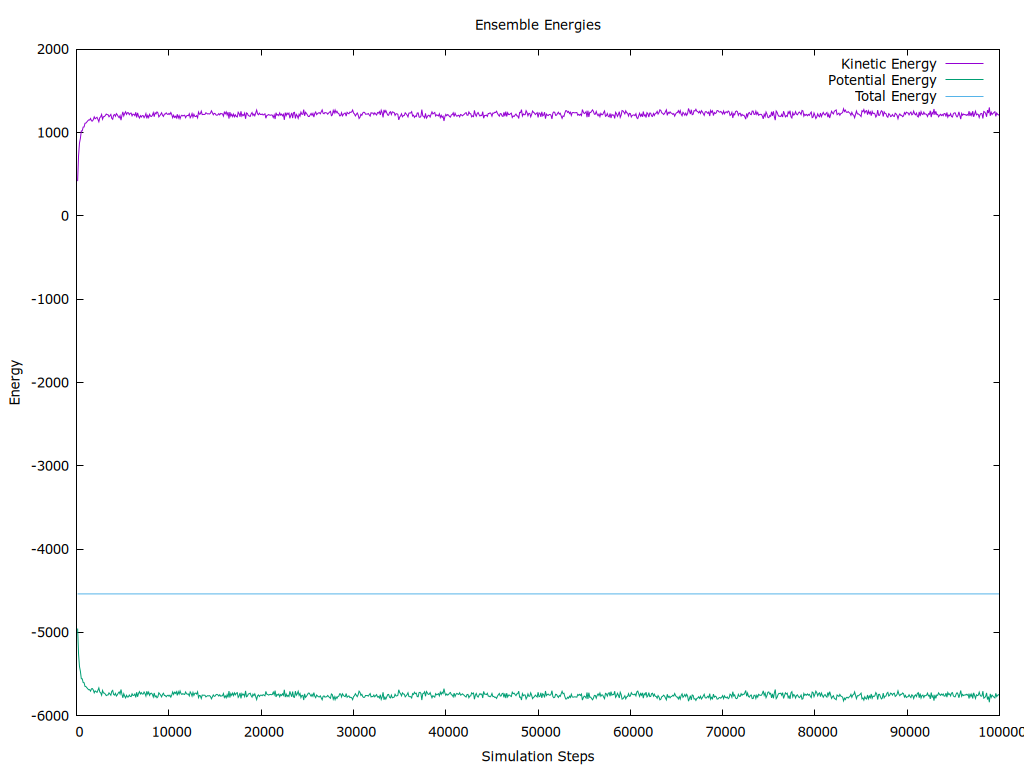
\includegraphics[width=.9\linewidth]{../../runs/nve_lammps_pair_style/plots/energy.png}
\end{center}
\subsection{Temperature and Velocity Distribution}
\label{sec:org3349f3e}
\begin{center}
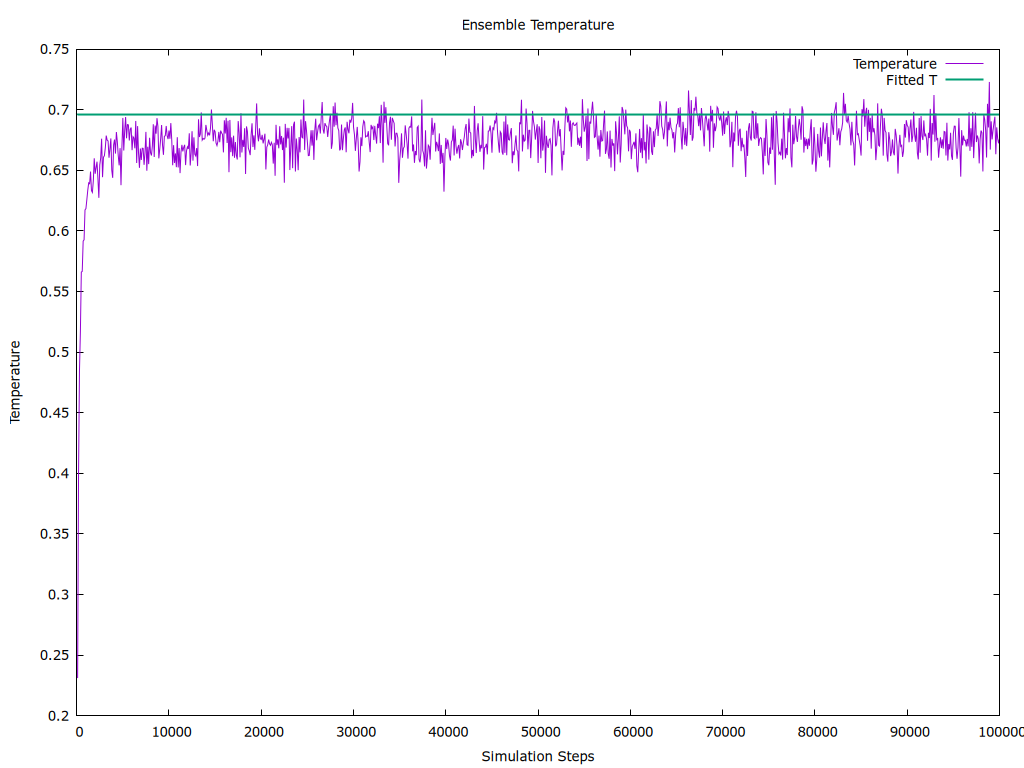
\includegraphics[width=.9\linewidth]{../../runs/nve_lammps_pair_style/plots/temperature.png}
\end{center}

\begin{center}
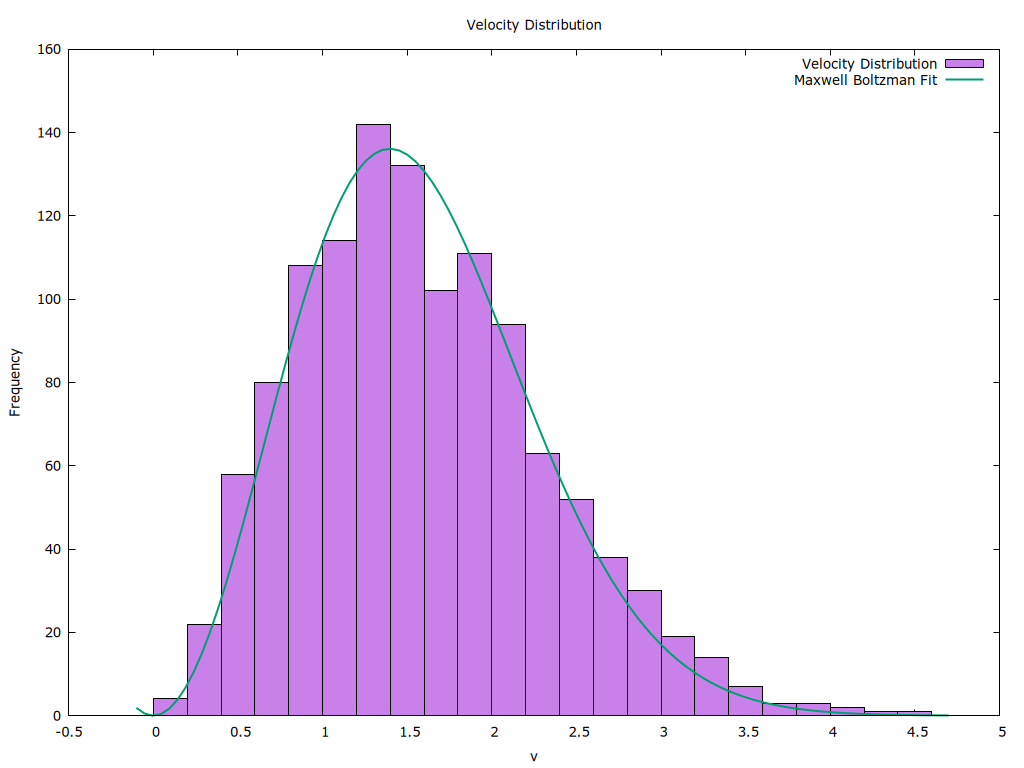
\includegraphics[width=.9\linewidth]{../../runs/nve_lammps_pair_style/plots/velocity_dist.png}
\end{center}
\subsection{Pressure}
\label{sec:org568d20d}
\begin{center}
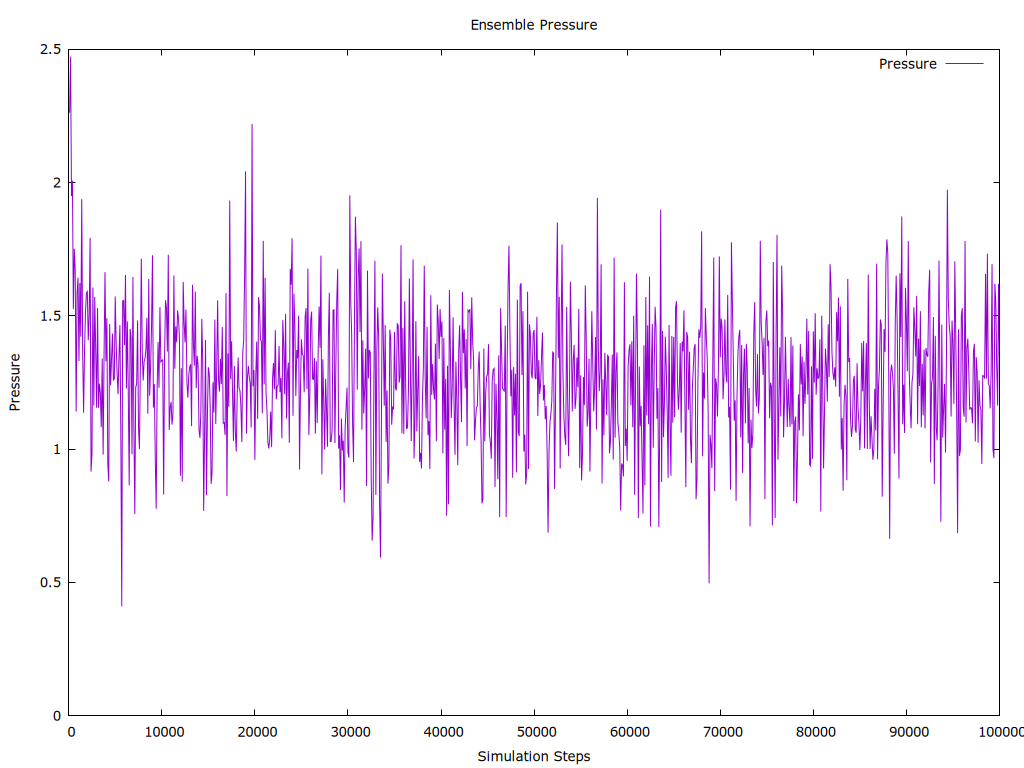
\includegraphics[width=.9\linewidth]{../../runs/nve_lammps_pair_style/plots/pressure.png}
\end{center}
\subsection{Ensemble Momentum and COM Velocity}
\label{sec:org693b4ab}
\begin{center}
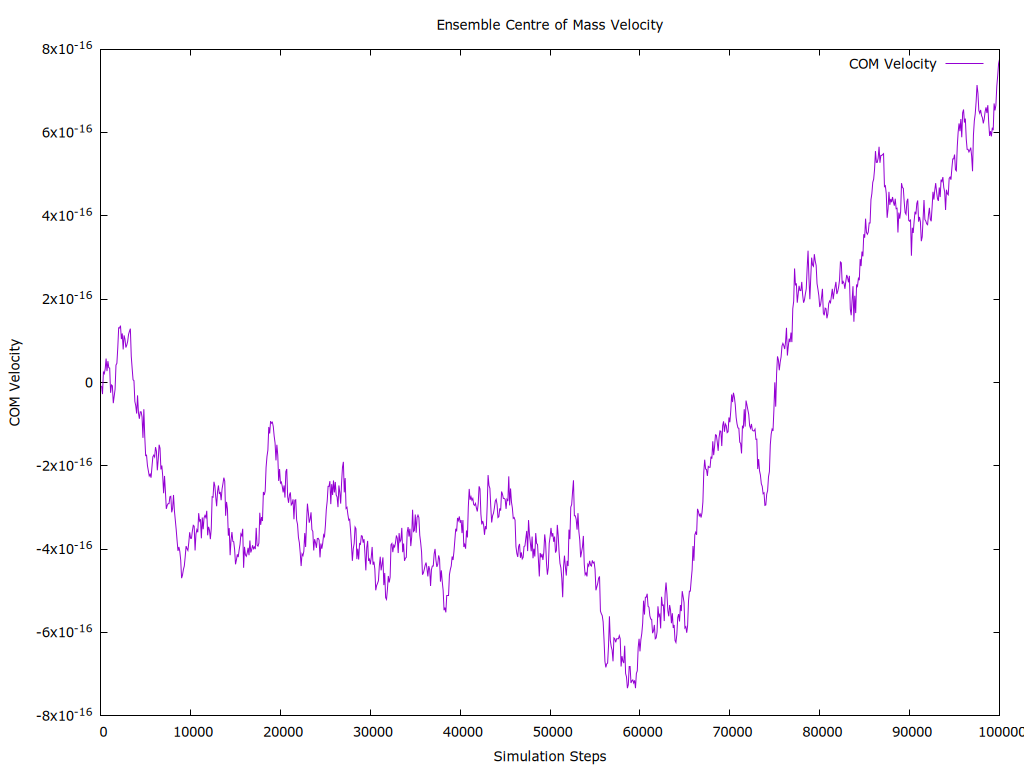
\includegraphics[width=.9\linewidth]{../../runs/nve_lammps_pair_style/plots/com_velocity.png}
\end{center}

\begin{center}
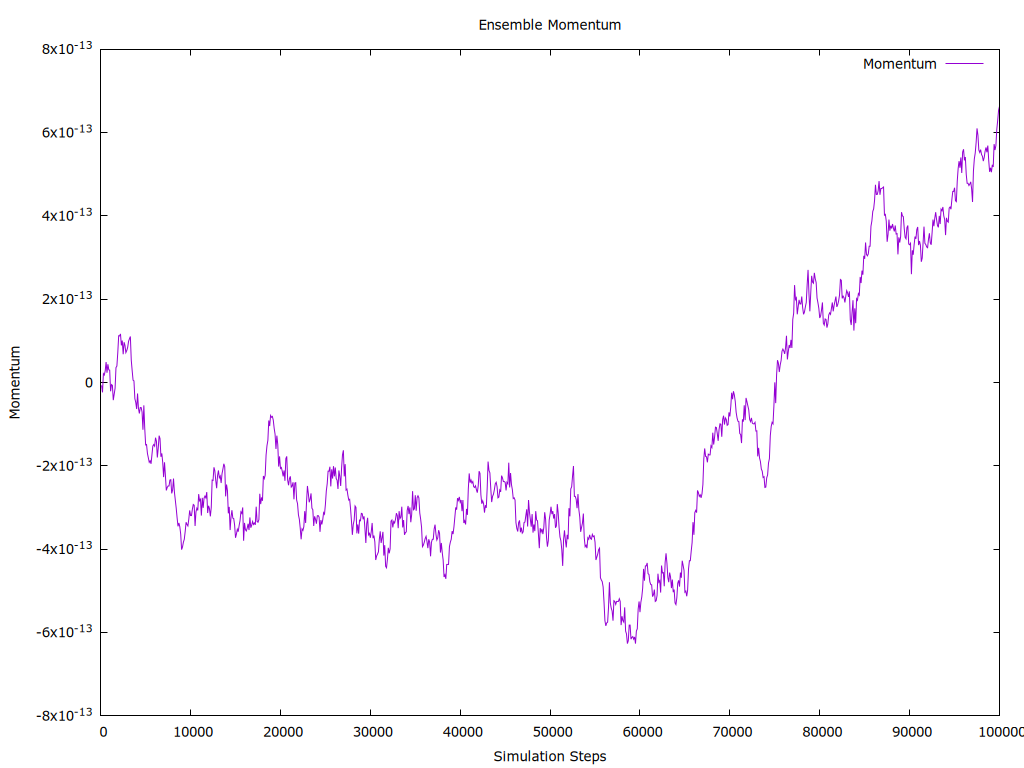
\includegraphics[width=.9\linewidth]{../../runs/nve_lammps_pair_style/plots/momentum.png}
\end{center}
\section{Cooling Checks}
\label{sec:orge757012}
\subsection{Parameters}
\label{sec:org767175a}
\begin{itemize}
\item Initial NVE Temperature \(T_{NVE}\)
\item Thermalize (Nose-Hover) to \(T_f + 500K = T^*_f + 0.07\)
\item Cooling to \(T_f\) in steps. Each cooling step involves rapid cooling for \(n_c\), followed by thermalization (Nose-Hover) for \(n_t\)
\end{itemize}
\subsection{\(T^*_f = 0.28, \quad N = 501\)}
\label{sec:org97cb660}
\subsubsection{Energy}
\label{sec:org4a016e6}
\begin{center}
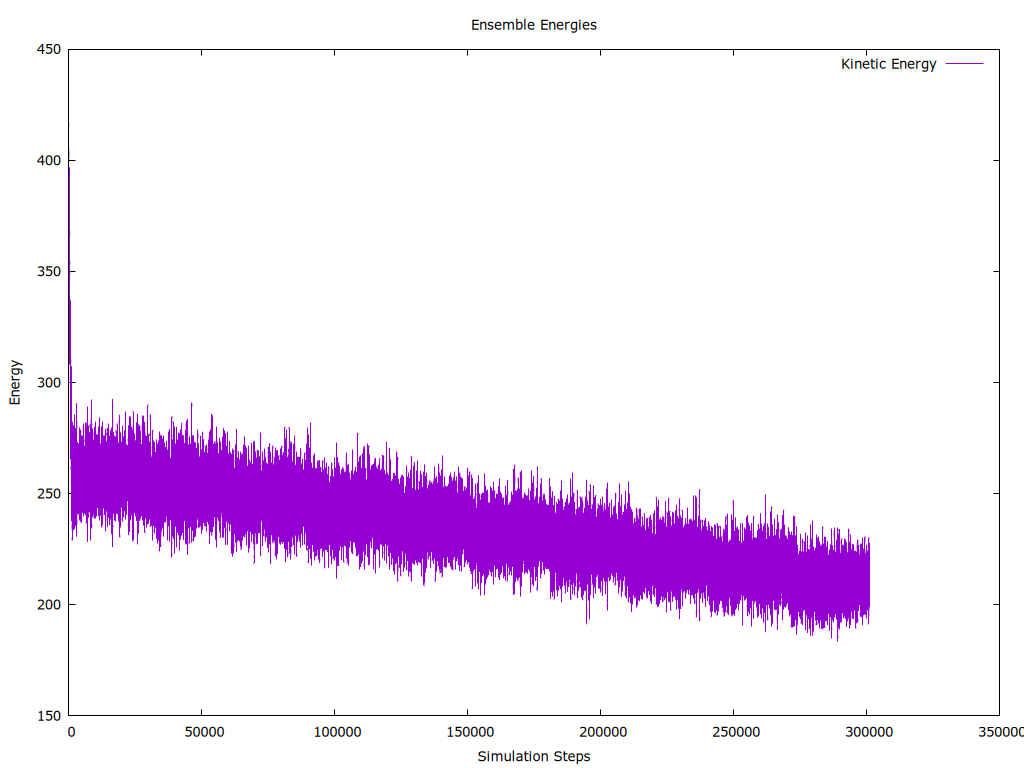
\includegraphics[width=.9\linewidth]{../../runs/nvt_cool_sample/plots/N_501_T_0.28/ke.png}
\end{center}

\begin{center}
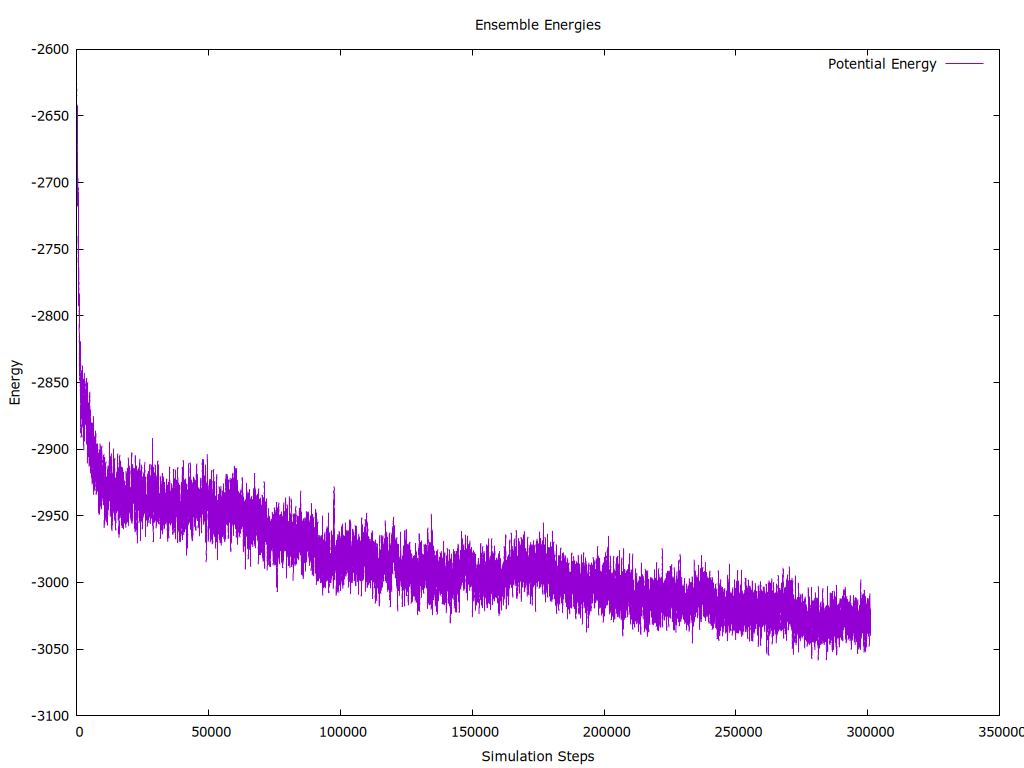
\includegraphics[width=.9\linewidth]{../../runs/nvt_cool_sample/plots/N_501_T_0.28/pe.png}
\end{center}

\begin{center}
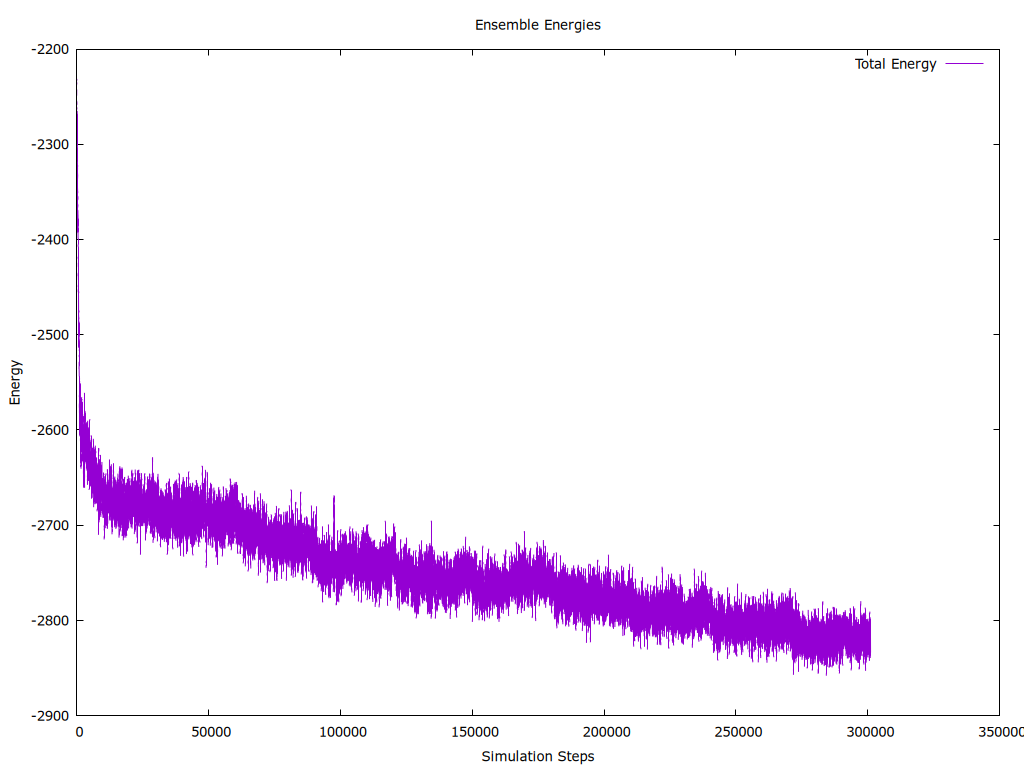
\includegraphics[width=.9\linewidth]{../../runs/nvt_cool_sample/plots/N_501_T_0.28/te.png}
\end{center}
\subsubsection{Temperature}
\label{sec:org0052518}
\begin{center}
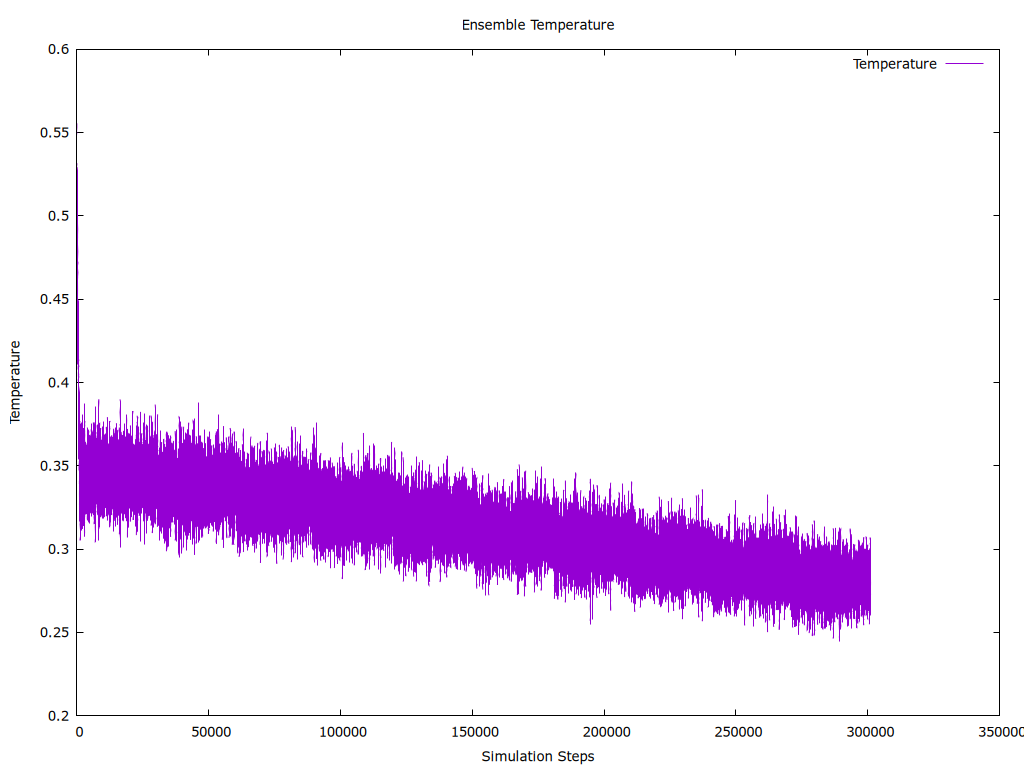
\includegraphics[width=.9\linewidth]{../../runs/nvt_cool_sample/plots/N_501_T_0.28/temperature.png}
\end{center}
\subsubsection{Pressure}
\label{sec:org8a5d188}
\begin{center}
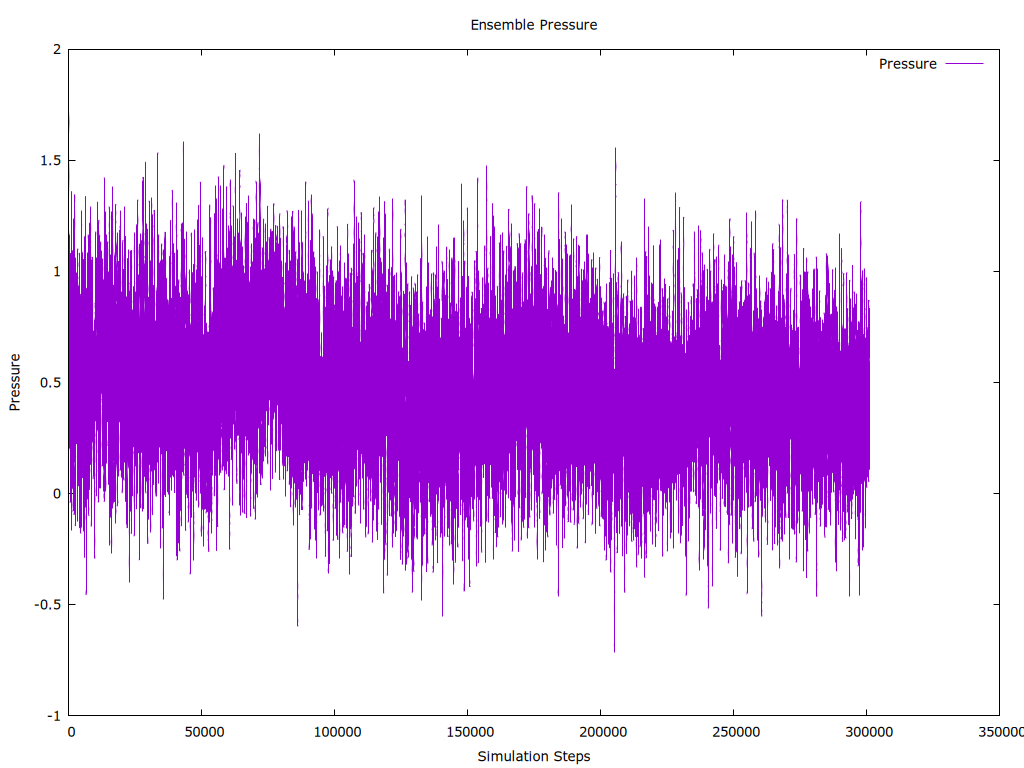
\includegraphics[width=.9\linewidth]{../../runs/nvt_cool_sample/plots/N_501_T_0.28/pressure.png}
\end{center}
\subsubsection{Average NVT Temperature vs KE}
\label{sec:org4d65822}
\begin{center}
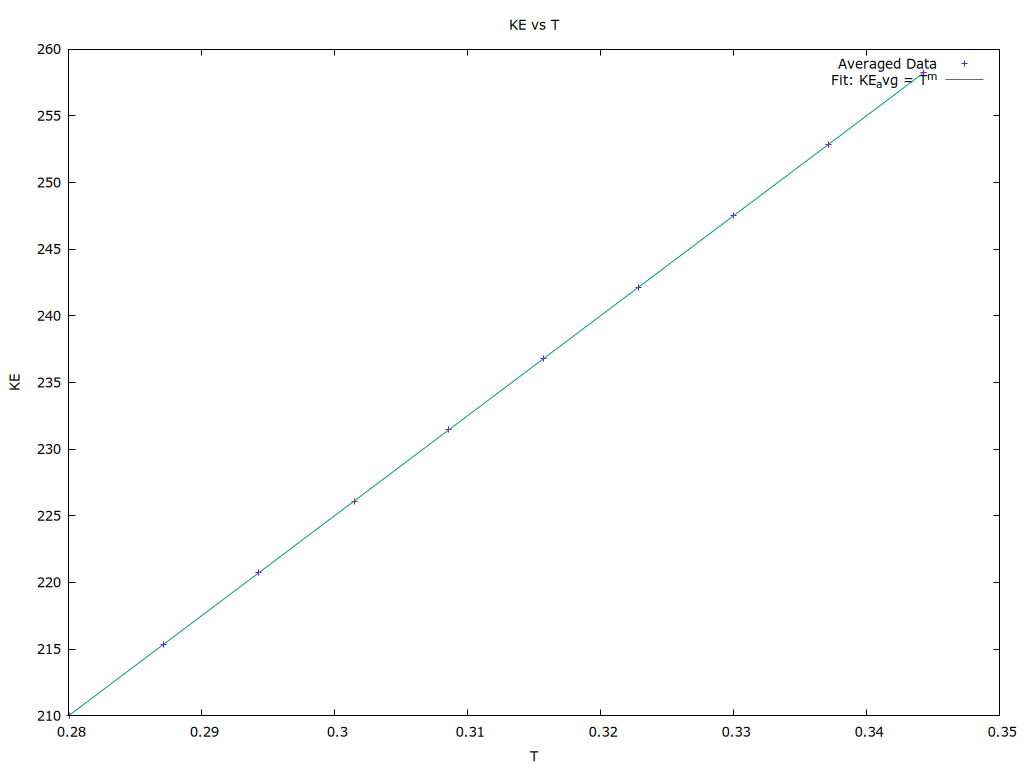
\includegraphics[width=.9\linewidth]{../../runs/nvt_cool_sample/plots/N_501_T_0.28/TvsKE.png}
\end{center}

\begin{align*}
KE = \alpha T ^ m, \quad m = 0.99, \quad \alpha = 749.99
\end{align*}
\section{NVT Checks}
\label{sec:org49fe76d}
\subsection{Coslovich and Pastore RDF Check \(T^*_f = 0.28, \quad N = 501, \quad \rho = 1.655\)}
\label{sec:org79c8fba}
\subsubsection{\(g_{11}(r)\)}
\label{sec:orgcbb079f}
\begin{center}
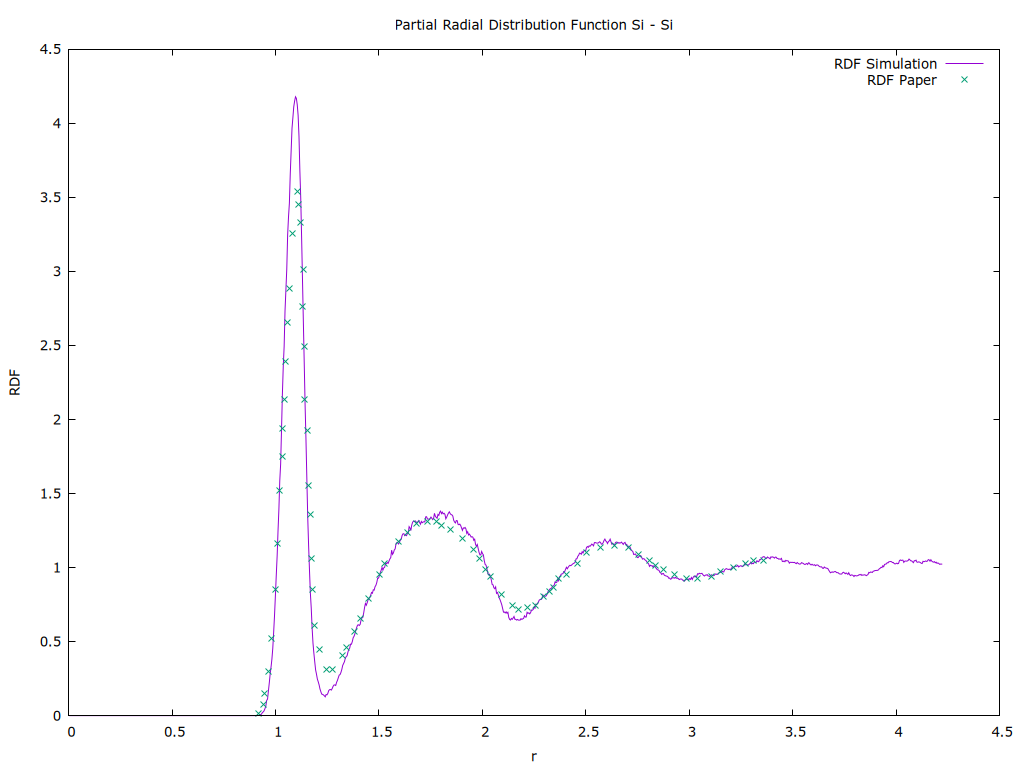
\includegraphics[width=.9\linewidth]{../../runs/nvt_cool_sample_rdf/plots/rdf_11.png}
\end{center}
\subsubsection{\(g_{12}(r)\)}
\label{sec:org0c784f7}

\begin{center}
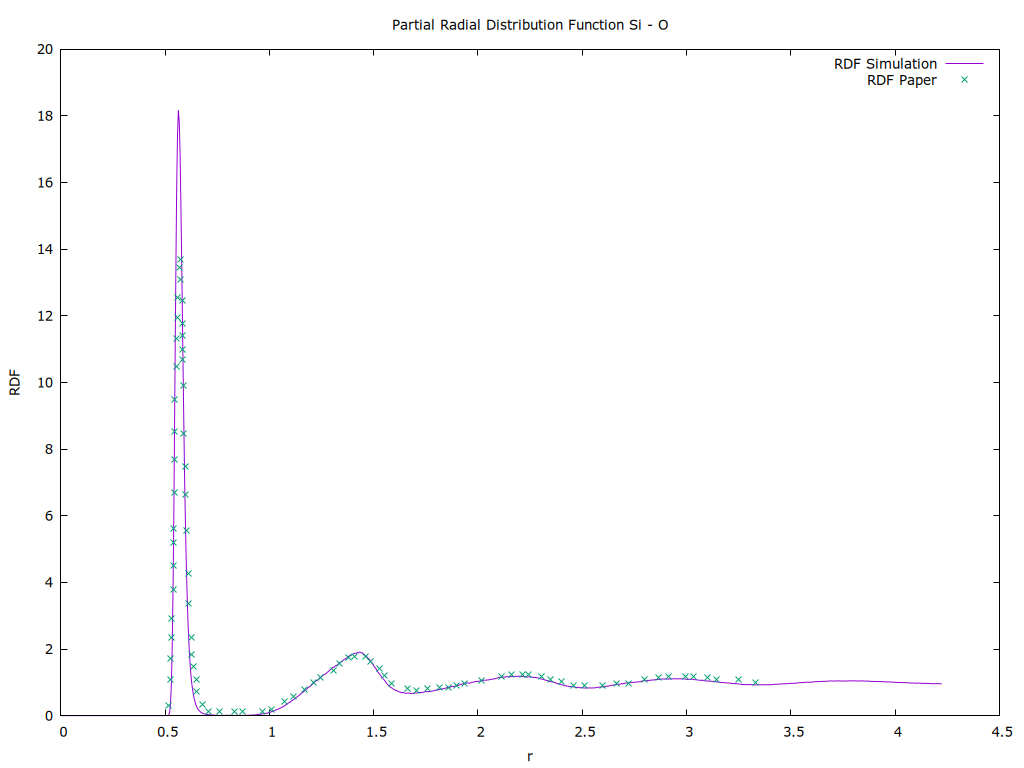
\includegraphics[width=.9\linewidth]{../../runs/nvt_cool_sample_rdf/plots/rdf_12.png}
\end{center}
\subsubsection{\(g_{22}(r)\)}
\label{sec:orgb4307b8}

\begin{center}
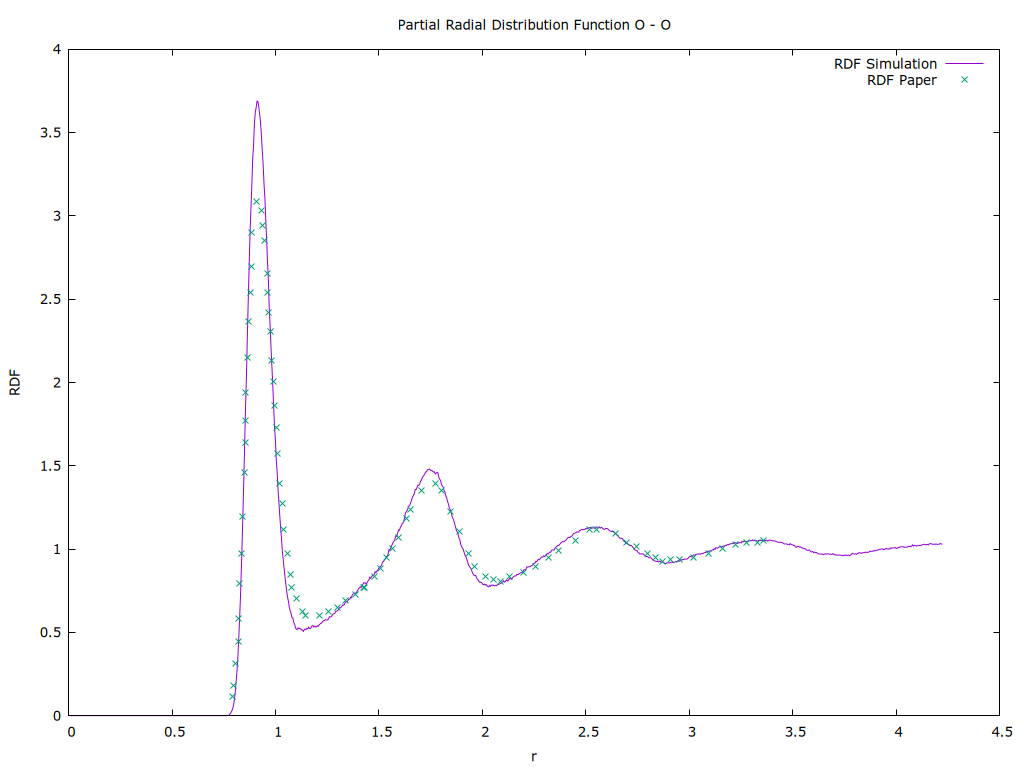
\includegraphics[width=.9\linewidth]{../../runs/nvt_cool_sample_rdf/plots/rdf_22.png}
\end{center}
\subsubsection{Density Check}
\label{sec:org61e2e94}
\begin{enumerate}
\item \(N = 501, \quad \rho = 1.655\)
\label{sec:orgbb879d4}

\begin{align*}
z_{}(R = 4.22113) = 522.054 \\
R_0 = 4.22113 \implies \frac{4}{3}\pi R_0^3 = 315.047 \\
N_{sim} = 501, \quad \rho = 1.655 \\
\implies L = 6.71449326567 \implies L^3 = 302.718 \\
\end{align*}

\begin{align*}
\rho = \frac{N + 1}{L^3} = \frac{z(R_0)}{\frac{4}{3}\pi R_0^3} = 1.657 \\
\implies N + 1 = 501.7 \implies N = 500.7 \approx 501
\end{align*}
\end{enumerate}
\end{document}
